\chapter[Cosmic-Rays]{\centering Cosmic-Rays \\}\label{Ch:Cosmic-rays}

\section{History of Cosmic-Rays}

First detection of ionizing radiation. 

1785: Coulomb found that 
electroscopes can spontaneously 
discharge by the action of the air 
and not by defective insulation

1835: Faraday confirms the 
observation by Coulomb, with 
better insulation technology

1879: Crookes measures that the 
speed of discharge of an 
electroscope decreased when 
pressure was reduced 

\section{Energy Spectrum and Mass composition}

\begin{figure}[hp]
\centering
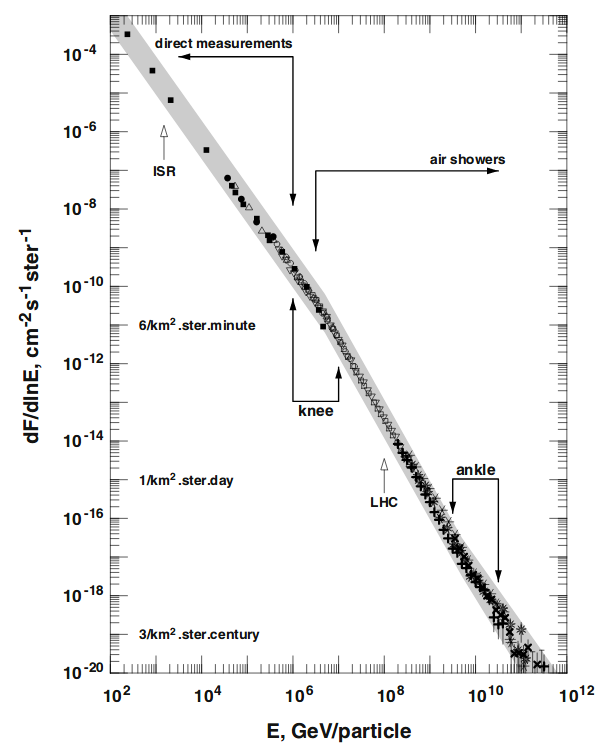
\includegraphics[width=\textwidth]{chapters/pix/CosmicRay_Spectrum.png}
\caption{Measured energy spectrum of cosmic-rays from 100 GeV up to the highest detected energy.}
\label{fig:CR_Spectrum}
\end{figure}

Cosmic-rays have been detected over a large range of energies from GeV (10$^9$ \ eV) to above EeV (10$^18$ \ eV). Spectrum in Figure \ref{fig:CR_Spectrum} shows the break at the knee and ankle and which type of experiments are most suited to measurement each part. Cosmic-ray spectrum starts out at E$^{-2}$ \ and can be as steep as E$^{-2.7}$ at the highest energies.

Cosmic-rays can consist of protons to iron. 

\section{Production Method and Sources}

Supernova explosions 

AGN jets

other energetic processes

dark matter annihilations.